%%%%%%%%%%%%%%%%%%%%%%%%%%%%%%%%%%%%%%%%%
% Beamer Presentation
% LaTeX Template
% Version 1.0 (10/11/12)
%
% This template has been downloaded from:
% http://www.LaTeXTemplates.com
%
% License:
% CC BY-NC-SA 3.0 (http://creativecommons.org/licenses/by-nc-sa/3.0/)
%
%%%%%%%%%%%%%%%%%%%%%%%%%%%%%%%%%%%%%%%%%

%----------------------------------------------------------------------------------------
%	PACKAGES AND THEMES
%----------------------------------------------------------------------------------------

\documentclass{beamer}
\setbeamercovered{transparent}
\setbeamercolor{local structure}{fg=black}
\setbeamertemplate{caption}{\raggedright\insertcaption\par}
\usefonttheme[onlymath]{serif}

\mode<presentation> {
	
	% The Beamer class comes with a number of default slide themes
	% which change the colors and layouts of slides. Below this is a list
	% of all the themes, uncomment each in turn to see what they look like.
	
	%\usetheme{default}
	%\usetheme{AnnArbor}
	%\usetheme{Antibes}
	%\usetheme{Bergen}
	%\usetheme{Berkeley}
	%\usetheme{Berlin}
	%\usetheme{Boadilla}
	\usetheme{CambridgeUS}
	%\usetheme{Copenhagen}
	%\usetheme{Darmstadt}
	%\usetheme{Dresden}
	%\usetheme{Frankfurt}
	%\usetheme{Goettingen}
	%\usetheme{Hannover}
	%\usetheme{Ilmenau}
	%\usetheme{JuanLesPins}
	%\usetheme{Luebeck}
	%\usetheme{Madrid}
	%\usetheme{Malmoe}
	%\usetheme{Marburg}
	%\usetheme{Montpellier}
	%\usetheme{PaloAlto}
	%\usetheme{Pittsburgh}
	%\usetheme{Rochester}
	%\usetheme{Singapore}
	%\usetheme{Szeged}
	%\usetheme{Warsaw}
	
	% As well as themes, the Beamer class has a number of color themes
	% for any slide theme. Uncomment each of these in turn to see how it
	% changes the colors of your current slide theme.
	
	%\usecolortheme{albatross}
	%\usecolortheme{beaver}
	%\usecolortheme{beetle}
	%\usecolortheme{crane}
	%\usecolortheme{dolphin}
	%\usecolortheme{dove}
	%\usecolortheme{fly}
	%\usecolortheme{lily}
	\usecolortheme{orchid}
	%\usecolortheme{rose}
	%\usecolortheme{seagull}
	%\usecolortheme{seahorse}
	%\usecolortheme{whale}
	%\usecolortheme{wolverine}
	
	%\setbeamertemplate{footline} % To remove the footer line in all slides uncomment this line
	%\setbeamertemplate{footline}[page number] % To replace the footer line in all slides with a simple slide count uncomment this line
	
	%\setbeamertemplate{navigation symbols}{} % To remove the navigation symbols from the bottom of all slides uncomment this line
}

\usepackage{graphicx} % Allows including images
\usepackage{booktabs} % Allows the use of \toprule, \midrule and \bottomrule in tables
\usepackage{caption}
\captionsetup{font=scriptsize,labelfont=scriptsize}
\usepackage{amssymb}
\usepackage{bm}
\usepackage[colorinlistoftodos,prependcaption,textsize=small]{todonotes}                                                                                                                 

%----------------------------------------------------------------------------------------
%	TITLE PAGE
%----------------------------------------------------------------------------------------

\title[Large-Scale Data Analysis Techniques]{A Review on Multi-Label Learning Algorithms} % The short title appears at the bottom of every slide, the full title is only on the title page

\author[Sissy Themeli, Nikiforos Pittaras]{Min-Ling Zhang and Zhi-Hua Zhou} % Your name
\institute[DI-UOA] % Your institution as it will appear on the bottom of every slide, may be shorthand to save space
{
	IEEE TRANSACTIONS ON KNOWLEDGE AND DATA ENGINEERING\\ % Your institution for the title page
	\medskip
}
\date{\today} % Date, can be changed to a custom date

\begin{document}
	
	\begin{frame}
	\titlepage % Print the title page as the first slide
\end{frame}

\begin{frame}
\frametitle{Overview} % Table of contents slide, comment this block out to remove it
\tableofcontents % Throughout your presentation, if you choose to use \section{} and \subsection{} commands, these will automatically be printed on this slide as an overview of your presentation
%\setbeamercolor{section in toc}{fg=black}
%\setbeamercolor{subsection in toc}{fg=black}
\end{frame}

%----------------------------------------------------------------------------------------
%	PRESENTATION SLIDES
%----------------------------------------------------------------------------------------

%------------------------------------------------
\section{Introduction} % Sections can be created in order to organize your presentation into discrete blocks, all sections and subsections are automatically printed in the table of contents as an overview of the talk
\subsection{Problem Definition}
\begin{frame}
\frametitle{\insertsection : \insertsubsection}
Single-label supervised learning
\begin{itemize}
	\item Applied to classification
	\item Supervised: Given dataset $\{ (x_i, y_i)\}, i = 1, \dots N, x \in X, y \in Y$
	\item Goal is to learn a model $f: X \rightarrow Y$
\end{itemize}

Multi-label supervised learning
\begin{itemize}
	\item Multiple labels per instance: $\{ (x_i, \bm{y}_i)\}, i = 1, \dots N, x \in X, \bm{y} \in \mathbb{P}(Y)$
	\item Learn a model $f: X \times Y \rightarrow r$ where $r\in \mathbb{R}$ is the confidence that $y_i$ characterizes $x_i$
	\item For classification, assume that $x_i$ belongs to $y_i$ if $r \ge $ $t(x_i)$

		\begin{itemize}
			\item $t(\cdot)$ can be a predetermined constant function or learned from $X$
		\end{itemize}

\end{itemize}
TODO: Include stuff about multi-labeled dataset characterization?
\end{frame}

%------------------------------------------------
\subsection{Algorithm Strategies}
\begin{frame}
\frametitle{\insertsection : \insertsubsection}
Label search space $\mathbb{S_Y}$ grows exponentially as a function of $|Y|$: 
\begin{itemize}
	\item e.g. for $|Y|=20, |\mathbb{S_Y}| = 2 ^ {|\mathbb{P(Y)}|} = 2^{20} \ge 10^6$
\end{itemize}
Solution: integrate in the learning process potential label correlations.
This work examines algorithms grouped in three broad categories:

\begin{enumerate}
	\item First-order strategies
		\begin{itemize}
			\item Transform multi-labeled problem to multiple, single-label problems 
			\item Ignore label correlations 
			\item Simple, scalable, suboptimal
		\end{itemize}
	\item Second-order strategies
		\begin{itemize}
			\item Consider \emph{pairwise} label relations
			\item Good trade-off between generalization performance and scalability
			\item Lacking in some real-world applications
		\end{itemize} 
	\item Higher-order strategies
		\begin{itemize}
			\item Capture more complicated label interdependencies
			\item Strong modeling capabilities
			\item Computationally demanding, less scalable
		\end{itemize}

\end{enumerate}
\end{frame}

%------------------------------------------------
\subsection{Evaluation Metrics}
\begin{frame}
\frametitle{\insertsection : \insertsubsection}
Need for more complicated evaluation than traditional supervised learning(accuracy, F-measure etc). There are 2 metrics categories 
	\begin{itemize}
		\item \emph{Example-based: }Evaluates system's performance on each example and returns the mean value. 
		\begin{itemize}
			\item \emph{From classification perspective:} $Subset Accuracy$, $Hamming Loss$, $accuracy_{exam}$, $precision_{exam}$, $recall_{exam}$, $F^\beta_{exam}$
			\item \emph{From ranking perspective:} one-error, coverage, ranking loss, average precision
		\end{itemize}
		\item \emph{Label-based: }Evaluates system's performance on each class label separately and returns macro/micro averaged value across all class labels
		\begin{itemize}
			\item From classification perspective: $B_{macro}$, $B_{micro}$
			\item From ranking perspective: $AUC_{macro}$, $AUC_{micro}$
		\end{itemize}
	\end{itemize}
TODO: theoretical results?
\end{frame}
%------------------------------------------------
\section{Multi-label Learning Algorithms}
%------------------------------------------------

\subsection{Simple Categorization}

\begin{frame}
\frametitle{\insertsection : \insertsubsection}

Assume multi-label classification problem with $q$ possible class labels $Y=\{y_1, \dots y_q\}$

Group algorithms in two categories:
\begin{itemize}
	\item \emph{Problem Transformation Methods: }Transform the learning problem into other well-established learning scenarios (fit data to algorithm philosophy)
	\item \emph{Algorithm Adaptation Methods: }Adapt popular learning techniques to deal with multi-label data directly (fit algorithm to data philosophy)
\end{itemize}
\end{frame}


%------------------------------------------------

\begin{frame}
\frametitle{\insertsection : \insertsubsection}
\begin{figure}
	\begin{center}
		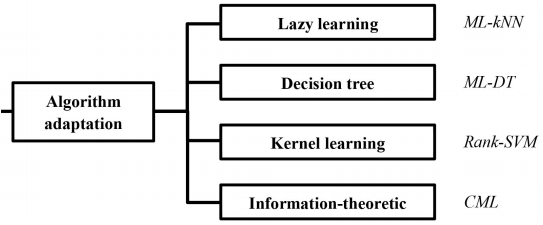
\includegraphics[scale = 0.75]{images/aa.png}
	\end{center}
\end{figure}
\end{frame}

\begin{frame}
\frametitle{\insertsection : \insertsubsection}
\begin{figure}
	\begin{center}
		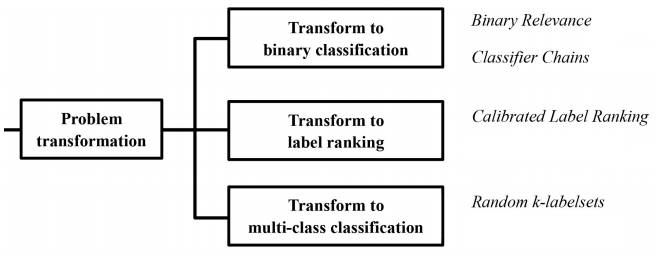
\includegraphics[scale = 0.7]{images/pt.png}
	\end{center}
\end{figure}
\end{frame}

%------------------------------------------------
\subsection{Problem Transformation Methods}
%------------------------------------------------
\begin{frame}
\Huge{\centerline{Problem Transformation Methods}}
\end{frame}
%------------------------------------------------
\begin{frame}
\frametitle{Binary Relevance}

\begin{itemize}
	\item Decompose to $q$ independent binary classification problems, $h_i(x)$
	\item Cross-train on $q$ binary training sets (one for each $y_i$)
	\item Predict labels of unseen $x$ by evaluating each classifier $h_i(x)$
	\item Output labels where  $h_i(x) > 0$ else $\underset{1 \geq i \geq q}{argmax} \{h_i(x))\}$ 
\end{itemize}

Pros \& cons:
\begin{itemize}
	\item Simple, parallelizable
	\item Sensitive to class-imbalanced data
	\item Ignores label correlations (first-order method)
\end{itemize}

\end{frame}
%------------------------------------------------

\begin{frame}
\frametitle{Classifier chains}
\begin{itemize}
	\item High-order approach algorithm
	\item Transform the problem into a chain of binary classification problems
	\item Build subsequent binary classifiers upon the predictions of preceding ones
	\item A permutation function is used to specify an order to the labels
	\item Binary training set
constructed by appending each instance with its relevance
to those labels
	\item Predict relevant labels for unknown instances by iteratively traversing the classifier chain
\end{itemize}

Pros \& cons:
\begin{itemize}
	\item Effectiveness largely affected by the ordering
	\item Exploitation of label correlations
	\item Does not support parallel implementation
\end{itemize}
\end{frame}
%------------------------------------------------

\begin{frame}
\frametitle{Calibrated Label Ranking}
\begin{itemize}
	\item Second-order approach algorithm
	\item Transform the problem into a label ranking problem
	\item Ranking implemented by pairwise comparison techniques
	\item For $q$ labels, generate $q(q-1)/2$ binary classifiers by pairwise comparison
	\item Construct training set per label pairs considering the example's relevance
	\item For unknown instance, get the overall classifiers' votes
	\item Virtual label $y_v$ as thresholding parameter
\end{itemize}
Pros \& cons:
\begin{itemize}
	\item Smooth the class-imbalance
	\item Classifier's number grows from linear to quadratic scale
	\begin{itemize}
		\item Improvement: Exact or approximate pruning to reduce classifier's number to be queried
	\end{itemize}
\end{itemize}
\end{frame}
%------------------------------------------------
\begin{frame}
\frametitle{Random k-Labelsets}
\begin{itemize}
	\item High-order approach algorithm
	\item Decompose to an ensemble of multi-class classification problems
	\item Each component targets a random subset of $Y$, inducing a multi-class classifier by Label Powerset (LP) techniques
	\item Convert training set into a multi-class set, treating each label set as a new class
	\item Each example is reassigned with the mapped single-label participating in multi-class classifier induction
	\item For unknown $x$, counts the maximum and actual number of votes
	\item Label set is relevant when the actual number of votes exceeds
half of the maximum ones
\end{itemize}
Pros \& cons:
\begin{itemize}
	\item Incompleteness: predicts only label sets included in the training set
	\item Inefficiency: large $Y$ implies high training complexity.Improvement by combining LP and ensemble learning
\end{itemize}
\end{frame}
%------------------------------------------------
\subsection{Alogrithm Adaptation Methods}
%------------------------------------------------
\begin{frame}
\Huge{\centerline{Alogrithm Adaptation Methods}}
\end{frame}
%------------------------------------------------
\begin{frame}
\frametitle{Multi-Label k-Nearest Neighbour}
\begin{itemize}
	\item First-order approach algorithm, adapting knn techniques
	\item Maximum a posteriori (MAP) rule to make prediction by reasoning and embody label info in the neighbours
	\item For new instances, $N(x)$ represents the set of its knn (uses Euclidean distance)
	
\end{itemize}
\end{frame}

%------------------------------------------------
\begin{frame}
\frametitle{Multi-label Decision Tree}

\end{frame}
%------------------------------------------------
\begin{frame}
\frametitle{Ranking Support Vector Machine}

\end{frame}
%------------------------------------------------
\begin{frame}
\frametitle{Collective Multi-Label Classifier}

\end{frame}
%------------------------------------------------
\section{Related Learning Settings}
%------------------------------------------------

\begin{frame}
\frametitle{Related Learning Settings}
\begin{itemize}
\item 
\item 
\item 
\item 
\end{itemize}
\end{frame}

%------------------------------------------------
\section{Conclusion}
%------------------------------------------------
\begin{frame}
\frametitle{Conclusion}
\begin{itemize}
	\item 
\end{itemize}
\end{frame}

%------------------------------------------------
\section{The end}
\begin{frame}
\Huge{\centerline{Thank you}}
\end{frame}
%------------------------------------------------
\end{document} 
